\documentclass[aspectratio=169,11pt]{beamer}
\usetheme{Madrid}
\usecolortheme{dolphin}  % Friendlier color scheme

% Packages
\usepackage{graphicx}
\usepackage{tikz}
\usepackage{amsmath}
\usepackage{amssymb}
\usepackage{hyperref}
\usepackage{xcolor}
\usepackage{verbatim}
% \usepackage{emoji}  % Requires LuaTeX
\usepackage{animate}
\usepackage{multicol}
% \usepackage{tcolorbox}  % Commented out - causing issues with beamer

% TikZ libraries
\usetikzlibrary{shapes,arrows,positioning,calc,shadows,patterns}
\usetikzlibrary{decorations.pathreplacing,decorations.pathmorphing}

% Custom colors
\definecolor{radioblue}{RGB}{0,123,255}
\definecolor{radiogreen}{RGB}{40,167,69}
\definecolor{radioorange}{RGB}{255,133,27}
\definecolor{radiopurple}{RGB}{111,66,193}
\definecolor{radiogray}{RGB}{108,117,125}

% Custom commands for visual elements
\newcommand{\highlight}[1]{\colorbox{yellow!30}{#1}}
\newcommand{\important}[1]{\textcolor{radioblue}{\textbf{#1}}}
\newcommand{\tryitnow}[1]{\fcolorbox{radiogreen}{radiogreen!10}{\parbox{0.9\textwidth}{\textbf{Try This Now!} #1}}}

% Title Information
\title{Welcome to the World of Software Defined Radio}
\subtitle{A Beginner's Journey with GNU Radio}
\author{Your Friendly Workshop Instructor}
\institute{GRCon 2025}
\date{\today}

\begin{document}

% Title slide with welcoming design
\begin{frame}
\titlepage
\begin{center}
\Large\textcolor{radioblue}{Let's explore radio waves together!}
\end{center}
\end{frame}

% ============================================
% SECTION 1: WELCOME & MOTIVATION
% ============================================

\section{Welcome \& Why We're Here}

\begin{frame}{Welcome to Your SDR Journey!}
\begin{columns}
\column{0.6\textwidth}
\Large
\textbf{Today you will:}
\begin{itemize}
    \item Understand radio in a new way
    \item Build your first radio system
    \item See invisible signals around you
    \item Join a global community
\end{itemize}
\vspace{1em}
\normalsize
\textcolor{radiogreen}{No prior experience needed!}

\column{0.4\textwidth}
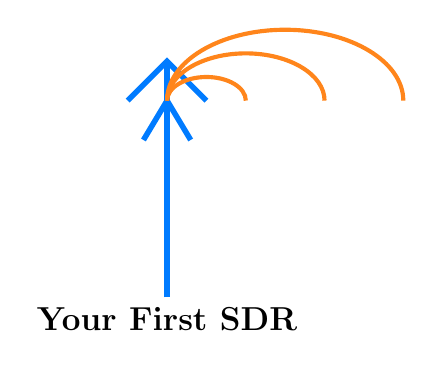
\begin{tikzpicture}
    % Simple radio tower illustration
    \draw[line width=2pt, radioblue] (0,0) -- (0,3);
    \draw[line width=2pt, radioblue] (-0.5,2.5) -- (0,3) -- (0.5,2.5);
    \draw[line width=2pt, radioblue] (-0.3,2) -- (0,2.5) -- (0.3,2);
    % Radio waves
    \foreach \i in {1,2,3} {
        \draw[radioorange, line width=1.5pt] (0,2.5) arc (180:0:\i*0.5 and \i*0.3);
    }
    \node[below] at (0,0) {\large\textbf{Your First SDR}};
\end{tikzpicture}
\end{columns}
\end{frame}

\begin{frame}{Why Learn Software Defined Radio?}
\begin{columns}[T]
\column{0.33\textwidth}
\begin{center}
\includegraphics[width=0.8\textwidth]{images/career_icon.png}
\textbf{Career Opportunities}
\end{center}
\begin{itemize}
    \item Telecom Industry
    \item Defense \& Security
    \item IoT Development
    \item Research Labs
\end{itemize}

\column{0.33\textwidth}
\begin{center}
\includegraphics[width=0.8\textwidth]{images/project_icon.png}
\textbf{Cool Projects}
\end{center}
\begin{itemize}
    \item Track Aircraft
    \item Receive Satellites
    \item Decode Weather
    \item Build Networks
\end{itemize}

\column{0.33\textwidth}
\begin{center}
\includegraphics[width=0.8\textwidth]{images/skill_icon.png}
\textbf{Valuable Skills}
\end{center}
\begin{itemize}
    \item Signal Processing
    \item Programming
    \item Problem Solving
    \item System Design
\end{itemize}
\end{columns}
\vspace{1em}
\begin{center}
\Large\textcolor{radioblue}{SDR is everywhere - from your phone to space stations!}
\end{center}
\end{frame}

\begin{frame}{What Can You Build with SDR?}
\begin{center}
\Large\textbf{Real Projects from Beginners Like You!}
\end{center}
\vspace{1em}
\begin{columns}
\column{0.25\textwidth}
\begin{center}
\textcolor{radioblue}{\Large\textbf{Week 1}}\\
FM Radio\\
Receiver
\end{center}

\column{0.25\textwidth}
\begin{center}
\textcolor{radiogreen}{\Large\textbf{Month 1}}\\
Aircraft\\
Tracker
\end{center}

\column{0.25\textwidth}
\begin{center}
\textcolor{radioorange}{\Large\textbf{Month 3}}\\
Weather\\
Satellite Decoder
\end{center}

\column{0.25\textwidth}
\begin{center}
\textcolor{radiopurple}{\Large\textbf{Month 6}}\\
Custom\\
Protocol
\end{center}
\end{columns}

\vspace{2em}
\begin{center}
\fcolorbox{radioblue}{blue!5}{\parbox{0.9\textwidth}{\centering
\large\textbf{Your Journey Starts Today!}}}
\end{center}
\end{frame}

\begin{frame}{Success Stories}
\begin{columns}
\column{0.5\textwidth}
\textbf{\large From the Community:}
\begin{itemize}
    \item \textbf{Sarah, Student:} "Built an emergency communication system for her town"
    \item \textbf{Mike, Hobbyist:} "Tracks ships entering the harbor"
    \item \textbf{Team Alpha:} "Won hackathon with SDR-based IoT security scanner"
\end{itemize}

\column{0.5\textwidth}
\textbf{\large Industry Applications:}
\begin{itemize}
    \item \textbf{SpaceX:} Satellite communications
    \item \textbf{Tesla:} Key fob security
    \item \textbf{Amazon:} Drone delivery systems
    \item \textbf{Your Company:} Next innovation?
\end{itemize}
\end{columns}
\vspace{1em}
\begin{center}
\Large\highlight{You're joining a revolution in wireless technology!}
\end{center}
\end{frame}

\begin{frame}{No Fear Zone}
\begin{center}
\Huge\textcolor{radiogreen}{Common Worries? We've Got You!}
\end{center}
\vspace{1em}
\begin{columns}
\column{0.5\textwidth}
\textbf{"I'm not good at math"}\\
\textcolor{radioblue}{$\rightarrow$ We'll use visual tools!}\\[0.5em]

\textbf{"I don't know programming"}\\
\textcolor{radioblue}{$\rightarrow$ Drag-and-drop to start!}\\[0.5em]

\textbf{"Hardware is expensive"}\\
\textcolor{radioblue}{$\rightarrow$ Start with \$30 RTL-SDR!}

\column{0.5\textwidth}
\textbf{"This seems complex"}\\
\textcolor{radiogreen}{$\rightarrow$ Step-by-step guidance!}\\[0.5em]

\textbf{"What if I break something?"}\\
\textcolor{radiogreen}{$\rightarrow$ Software can't break!}\\[0.5em]

\textbf{"I might fall behind"}\\
\textcolor{radiogreen}{$\rightarrow$ Work at your pace!}
\end{columns}
\vspace{1em}
\begin{center}
\fcolorbox{radioorange}{yellow!20}{\parbox{0.9\textwidth}{\centering
\large\textbf{Remember: Every expert was once a beginner!}}}
\end{center}
\end{frame}

% ============================================
% SECTION 2: RADIO FUNDAMENTALS
% ============================================

\section{Radio Basics - No PhD Required!}

\begin{frame}{What is a Radio Wave?}
\begin{center}
\Large\textbf{Think of it like ripples in a pond...}
\end{center}
\vspace{1em}
\begin{columns}
\column{0.5\textwidth}
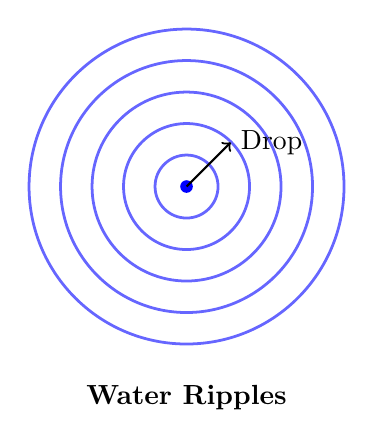
\begin{tikzpicture}[scale=0.8]
    % Pond ripples
    \foreach \r in {0.5,1,1.5,2,2.5} {
        \draw[blue!60, line width=1pt] (0,0) circle (\r);
    }
    \fill[blue] (0,0) circle (0.1);
    \node[below] at (0,-3) {\textbf{Water Ripples}};
    \draw[->, thick] (0,0) -- (0.7,0.7) node[right] {Drop};
\end{tikzpicture}

\column{0.5\textwidth}
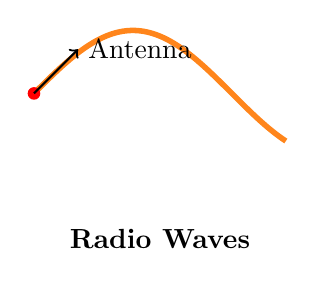
\begin{tikzpicture}[scale=0.8]
    % Radio waves
    \draw[radioorange, line width=2pt] plot[domain=0:4, samples=100] (\x, {sin(\x*180/pi)});
    \fill[red] (0,0) circle (0.1);
    \node[below] at (2,-2) {\textbf{Radio Waves}};
    \draw[->, thick] (0,0) -- (0.7,0.7) node[right] {Antenna};
\end{tikzpicture}
\end{columns}
\vspace{1em}
\begin{itemize}
    \item Radio waves are \important{invisible} electromagnetic ripples
    \item They travel at the \important{speed of light}
    \item They can carry \important{information} (music, data, video)
\end{itemize}
\end{frame}

\begin{frame}{Frequency and Wavelength - Pizza Analogy}
\begin{columns}
\column{0.6\textwidth}
\textbf{\Large Frequency = How Often}\\
Like pizza delivery frequency!
\begin{itemize}
    \item \textbf{Low frequency:} Pizza once a month
    \item \textbf{High frequency:} Pizza every day!
\end{itemize}
\vspace{1em}
\textbf{\Large Wavelength = How Big}\\
Like pizza sizes!
\begin{itemize}
    \item \textbf{Long wavelength:} Family size (travels far)
    \item \textbf{Short wavelength:} Personal (more data)
\end{itemize}

\column{0.4\textwidth}
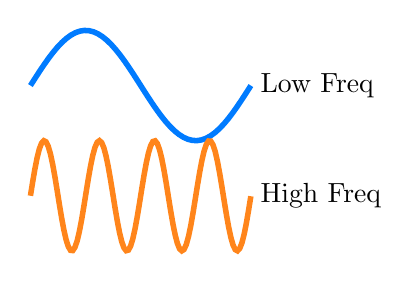
\begin{tikzpicture}[scale=0.7]
    % Low frequency wave
    \draw[radioblue, line width=2pt] plot[domain=0:4, samples=50] (\x, {sin(\x*90)});
    \node[right] at (4,0) {Low Freq};
    
    % High frequency wave
    \draw[radioorange, line width=2pt] plot[domain=0:4, samples=100] (\x, {-2+sin(\x*360)});
    \node[right] at (4,-2) {High Freq};
\end{tikzpicture}
\end{columns}
\vspace{1em}
\begin{center}\colorbox{yellow!20}{\parbox{0.9\textwidth}{
\textbf{Remember:} Higher frequency = More waves per second = Shorter wavelength
}}\end{center}
\end{frame}

\begin{frame}{The Radio Spectrum - Your Neighborhood}
\begin{center}
\textbf{\Large Think of the spectrum as a neighborhood with different zones}
\end{center}
\vspace{0.5em}
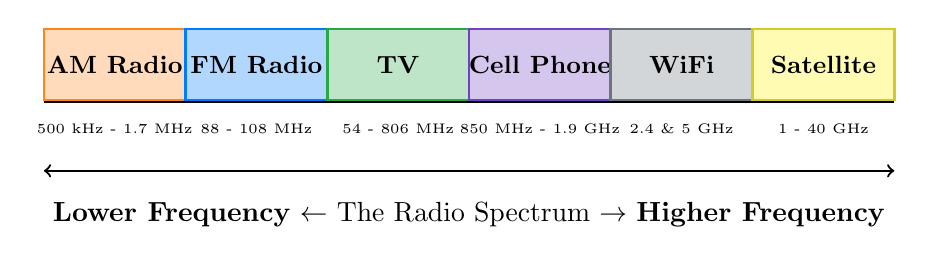
\begin{tikzpicture}[scale=0.9]
    % Spectrum visualization
    \draw[line width=2pt] (0,0) -- (12,0);
    
    % AM Radio
    \fill[radioorange!30] (0,0) rectangle (2,1);
    \draw[radioorange, line width=1pt] (0,0) rectangle (2,1);
    \node at (1,0.5) {\small\textbf{AM Radio}};
    \node[below] at (1,-0.2) {\tiny 500 kHz - 1.7 MHz};
    
    % FM Radio
    \fill[radioblue!30] (2,0) rectangle (4,1);
    \draw[radioblue, line width=1pt] (2,0) rectangle (4,1);
    \node at (3,0.5) {\small\textbf{FM Radio}};
    \node[below] at (3,-0.2) {\tiny 88 - 108 MHz};
    
    % TV
    \fill[radiogreen!30] (4,0) rectangle (6,1);
    \draw[radiogreen, line width=1pt] (4,0) rectangle (6,1);
    \node at (5,0.5) {\small\textbf{TV}};
    \node[below] at (5,-0.2) {\tiny 54 - 806 MHz};
    
    % Cell Phone
    \fill[radiopurple!30] (6,0) rectangle (8,1);
    \draw[radiopurple, line width=1pt] (6,0) rectangle (8,1);
    \node at (7,0.5) {\small\textbf{Cell Phone}};
    \node[below] at (7,-0.2) {\tiny 850 MHz - 1.9 GHz};
    
    % WiFi
    \fill[radiogray!30] (8,0) rectangle (10,1);
    \draw[radiogray, line width=1pt] (8,0) rectangle (10,1);
    \node at (9,0.5) {\small\textbf{WiFi}};
    \node[below] at (9,-0.2) {\tiny 2.4 \& 5 GHz};
    
    % Satellite
    \fill[yellow!30] (10,0) rectangle (12,1);
    \draw[yellow!80!black, line width=1pt] (10,0) rectangle (12,1);
    \node at (11,0.5) {\small\textbf{Satellite}};
    \node[below] at (11,-0.2) {\tiny 1 - 40 GHz};
    
    % Labels
    \draw[<->, thick] (0,-1) -- (12,-1);
    \node[below] at (6,-1.3) {\textbf{Lower Frequency} $\leftarrow$ The Radio Spectrum $\rightarrow$ \textbf{Higher Frequency}};
\end{tikzpicture}
\vspace{1em}
\begin{center}
\highlight{Each "zone" has specific rules and uses - just like residential vs commercial areas!}
\end{center}
\end{frame}

\begin{frame}{How Does Radio Communication Work?}
\begin{center}
\Large\textbf{It's Like Talking Across a Room!}
\end{center}
\vspace{1em}
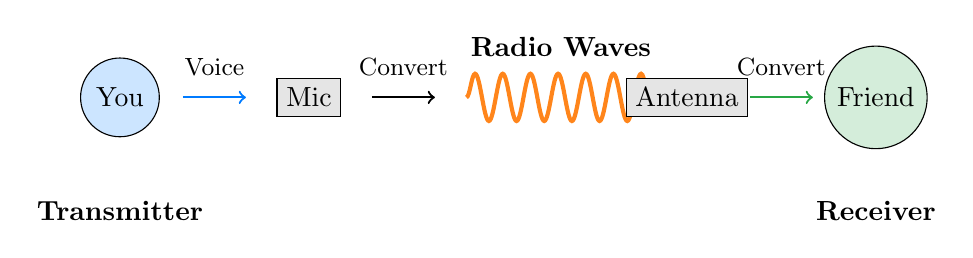
\begin{tikzpicture}[scale=0.8]
    % Person A (Transmitter)
    \node[draw, circle, minimum size=1cm, fill=radioblue!20] (personA) at (0,0) {You};
    \node[below] at (0,-1.5) {\textbf{Transmitter}};
    
    % Voice to Radio
    \draw[->, thick, radioblue] (1,0) -- (2,0);
    \node[above] at (1.5,0.2) {\small Voice};
    
    % Microphone
    \node[draw, rectangle, fill=gray!20] (mic) at (3,0) {Mic};
    
    % Processing
    \draw[->, thick] (4,0) -- (5,0);
    \node[above] at (4.5,0.2) {\small Convert};
    
    % Radio waves
    \draw[radioorange, line width=1.5pt, decorate, decoration={snake, amplitude=0.3cm}] (5.5,0) -- (8.5,0);
    \node[above] at (7,0.5) {\textbf{Radio Waves}};
    
    % Antenna
    \node[draw, rectangle, fill=gray!20] (speaker) at (9,0) {Antenna};
    
    % Radio to Voice
    \draw[->, thick, radiogreen] (10,0) -- (11,0);
    \node[above] at (10.5,0.2) {\small Convert};
    
    % Person B (Receiver)
    \node[draw, circle, minimum size=1cm, fill=radiogreen!20] (personB) at (12,0) {Friend};
    \node[below] at (12,-1.5) {\textbf{Receiver}};
\end{tikzpicture}
\vspace{1em}
\begin{columns}
\column{0.5\textwidth}
\textbf{Steps to Send:}
\begin{enumerate}
    \item Speak into microphone
    \item Convert sound to electricity
    \item Add to radio wave
    \item Transmit through antenna
\end{enumerate}

\column{0.5\textwidth}
\textbf{Steps to Receive:}
\begin{enumerate}
    \item Antenna catches waves
    \item Extract the sound signal
    \item Convert back to sound
    \item Listen through speaker
\end{enumerate}
\end{columns}
\end{frame}

\begin{frame}{Analog vs Digital - Letters vs Email}
\begin{columns}
\column{0.5\textwidth}
\begin{center}
\textbf{\Large Analog Radio}\\
\textcolor{radioblue}{Like Handwritten Letters}
\end{center}
\begin{itemize}
    \item Continuous, smooth signal
    \item Quality degrades with distance
    \item Simple but less flexible
    \item AM/FM radio, old TV
\end{itemize}
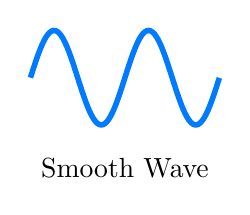
\begin{tikzpicture}[scale=0.6]
    \draw[radioblue, line width=2pt] plot[domain=0:4, samples=100] (\x, {sin(\x*180)});
    \node[below] at (2,-1.5) {Smooth Wave};
\end{tikzpicture}

\column{0.5\textwidth}
\begin{center}
\textbf{\Large Digital Radio}\\
\textcolor{radiogreen}{Like Email}
\end{center}
\begin{itemize}
    \item Discrete 1s and 0s
    \item Error correction possible
    \item Complex but powerful
    \item WiFi, Cell phones, GPS
\end{itemize}

\begin{tikzpicture}[scale=0.6]
    \draw[radiogreen, line width=2pt] (0,0) -- (0.5,0) -- (0.5,1) -- (1,1) -- (1,0) -- (1.5,0) -- (1.5,1) -- (2,1) -- (2,0) -- (2.5,0) -- (2.5,1) -- (3,1) -- (3,0) -- (3.5,0) -- (3.5,1) -- (4,1);
    \node[below] at (2,-1.5) {Digital Steps};
\end{tikzpicture}
\end{columns}
\vspace{1em}
\begin{center}\colorbox{yellow!20}{\parbox{0.9\textwidth}{
\centering
\textbf{SDR can do BOTH! That's the power of software!}
}}\end{center}
\end{frame}

\begin{frame}{Why "Software Defined"?}
\begin{columns}
\column{0.5\textwidth}
\begin{center}
\textbf{\Large Traditional Radio}\\
\textcolor{radiogray}{Hardware Does Everything}
\end{center}
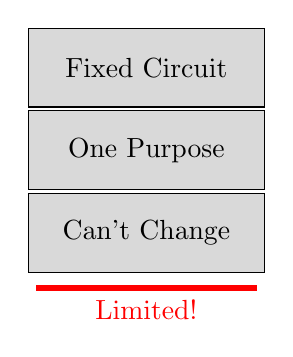
\begin{tikzpicture}[scale=0.7]
    \node[draw, rectangle, minimum width=3cm, minimum height=1cm, fill=gray!30] at (0,0) {Fixed Circuit};
    \node[draw, rectangle, minimum width=3cm, minimum height=1cm, fill=gray!30] at (0,-1.5) {One Purpose};
    \node[draw, rectangle, minimum width=3cm, minimum height=1cm, fill=gray!30] at (0,-3) {Can't Change};
    \draw[red, line width=2pt] (-2,-4) -- (2,-4) node[midway, below] {\textcolor{red}{Limited!}};
\end{tikzpicture}

\column{0.5\textwidth}
\begin{center}
\textbf{\Large Software Defined Radio}\\
\textcolor{radioblue}{Software Does the Magic}
\end{center}
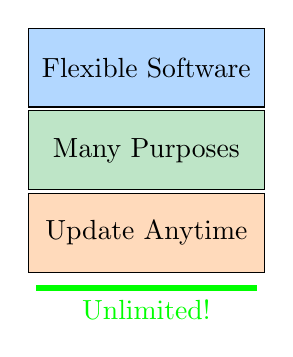
\begin{tikzpicture}[scale=0.7]
    \node[draw, rectangle, minimum width=3cm, minimum height=1cm, fill=radioblue!30] at (0,0) {Flexible Software};
    \node[draw, rectangle, minimum width=3cm, minimum height=1cm, fill=radiogreen!30] at (0,-1.5) {Many Purposes};
    \node[draw, rectangle, minimum width=3cm, minimum height=1cm, fill=radioorange!30] at (0,-3) {Update Anytime};
    \draw[green, line width=2pt] (-2,-4) -- (2,-4) node[midway, below] {\textcolor{green}{Unlimited!}};
\end{tikzpicture}
\end{columns}
\vspace{1em}
\begin{center}
\Large\highlight{One Device + Different Software = Many Radios!}
\end{center}
\end{frame}

\begin{frame}{Common Radio Terms Made Simple}
\begin{columns}
\column{0.5\textwidth}
\textbf{Essential Vocabulary:}
\begin{itemize}
    \item \textbf{Frequency:} Radio station number
    \item \textbf{Bandwidth:} How wide the road is
    \item \textbf{Modulation:} How we add information
    \item \textbf{Antenna:} Radio's ear and mouth
    \item \textbf{Gain:} Volume control
    \item \textbf{Noise:} Static/interference
\end{itemize}

\column{0.5\textwidth}
\textbf{In Daily Terms:}
\begin{itemize}
    \item \textbf{Spectrum:} Radio neighborhood
    \item \textbf{Channel:} Specific address
    \item \textbf{Signal:} The message
    \item \textbf{Carrier:} Delivery truck
    \item \textbf{Demodulation:} Unpacking the message
    \item \textbf{Filter:} Noise cancellation
\end{itemize}
\end{columns}
\vspace{1em}
\tryitnow{
Write down 3 radio terms you want to understand better - we'll cover them!
}
\end{frame}

\begin{frame}{Radio in Your Daily Life}
\begin{center}
\Large\textbf{You Use Radio Technology Every Day!}
\end{center}
\vspace{1em}
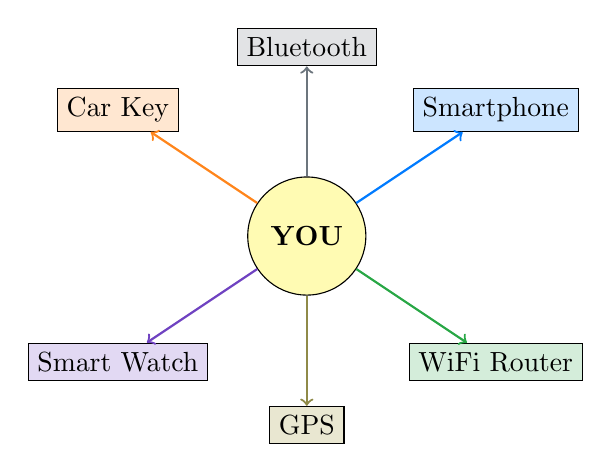
\begin{tikzpicture}[scale=0.8]
    % Center: You
    \node[draw, circle, minimum size=1.5cm, fill=yellow!30] (you) at (0,0) {\textbf{YOU}};
    
    % Surrounding devices
    \node[draw, rectangle, fill=radioblue!20] (phone) at (3,2) {Smartphone};
    \draw[->, thick, radioblue] (you) -- (phone);
    
    \node[draw, rectangle, fill=radiogreen!20] (wifi) at (3,-2) {WiFi Router};
    \draw[->, thick, radiogreen] (you) -- (wifi);
    
    \node[draw, rectangle, fill=radioorange!20] (car) at (-3,2) {Car Key};
    \draw[->, thick, radioorange] (you) -- (car);
    
    \node[draw, rectangle, fill=radiopurple!20] (watch) at (-3,-2) {Smart Watch};
    \draw[->, thick, radiopurple] (you) -- (watch);
    
    \node[draw, rectangle, fill=radiogray!20] (bluetooth) at (0,3) {Bluetooth};
    \draw[->, thick, radiogray] (you) -- (bluetooth);
    
    \node[draw, rectangle, fill=yellow!50!black!20] (gps) at (0,-3) {GPS};
    \draw[->, thick, yellow!50!black] (you) -- (gps);
\end{tikzpicture}
\vspace{0.5em}
\begin{center}
\highlight{Each uses different radio frequencies and protocols!}
\end{center}
\end{frame}

% ============================================
% SECTION 3: SDR CONCEPTS MADE SIMPLE
% ============================================

\section{Understanding SDR - The Easy Way}

\begin{frame}{SDR Building Blocks - Like LEGO!}
\begin{center}
\Large\textbf{Build Radios Like You Build with LEGO}
\end{center}
\vspace{1em}
\begin{columns}
\column{0.3\textwidth}
\begin{center}
\textcolor{radioblue}{\textbf{Sources}}\\
"Signal Creators"
\end{center}
\begin{itemize}
    \item Microphone
    \item Signal Generator
    \item File Player
    \item Hardware Input
\end{itemize}

\column{0.3\textwidth}
\begin{center}
\textcolor{radiogreen}{\textbf{Processors}}\\
"Signal Shapers"
\end{center}
\begin{itemize}
    \item Filters
    \item Amplifiers
    \item Modulators
    \item Decoders
\end{itemize}

\column{0.3\textwidth}
\begin{center}
\textcolor{radioorange}{\textbf{Sinks}}\\
"Signal Users"
\end{center}
\begin{itemize}
    \item Speaker
    \item Display
    \item File Saver
    \item Transmitter
\end{itemize}
\end{columns}
\vspace{1em}
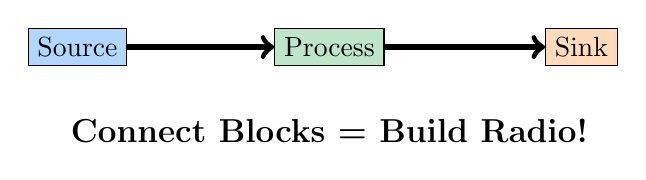
\begin{tikzpicture}[scale=0.8]
    \node[draw, rectangle, fill=radioblue!30] (source) at (0,0) {Source};
    \node[draw, rectangle, fill=radiogreen!30] (proc) at (4,0) {Process};
    \node[draw, rectangle, fill=radioorange!30] (sink) at (8,0) {Sink};
    \draw[->, line width=2pt] (source) -- (proc);
    \draw[->, line width=2pt] (proc) -- (sink);
    \node[below] at (4,-1) {\large\textbf{Connect Blocks = Build Radio!}};
\end{tikzpicture}
\end{frame}

\begin{frame}{Think of SDR Like a Music Studio}
\begin{columns}
\column{0.5\textwidth}
\textbf{\Large Music Studio}
\begin{itemize}
    \item \textbf{Microphone:} Input device
    \item \textbf{Mixer:} Combine sounds
    \item \textbf{Effects:} Modify audio
    \item \textbf{Speakers:} Output device
    \item \textbf{Recording:} Save to file
\end{itemize}

\column{0.5\textwidth}
\textbf{\Large SDR System}
\begin{itemize}
    \item \textbf{Antenna:} Input device
    \item \textbf{Adder:} Combine signals
    \item \textbf{Filters:} Modify signals
    \item \textbf{Display:} Output device
    \item \textbf{File Sink:} Save to file
\end{itemize}
\end{columns}
\vspace{1em}
\begin{center}\colorbox{yellow!20}{\parbox{0.9\textwidth}{
\centering
\large\textbf{If you can use audio software, you can use GNU Radio!}
}}\end{center}
\end{frame}

\begin{frame}{The Magic of IQ Data - Pizza Delivery Analogy}
\begin{center}
\Large\textbf{IQ Data = Complete Address System}
\end{center}
\vspace{1em}
\begin{columns}
\column{0.5\textwidth}
\textbf{Regular (Real) Signal:}\\
Like giving only street name
\begin{itemize}
    \item "Main Street"
    \item Missing information
    \item Can't find exact location
    \item Limited possibilities
\end{itemize}

\column{0.5\textwidth}
\textbf{IQ (Complex) Signal:}\\
Like giving full address
\begin{itemize}
    \item "123 Main Street, Apt 4B"
    \item Complete information
    \item Exact location
    \item All possibilities
\end{itemize}
\end{columns}
\vspace{1em}
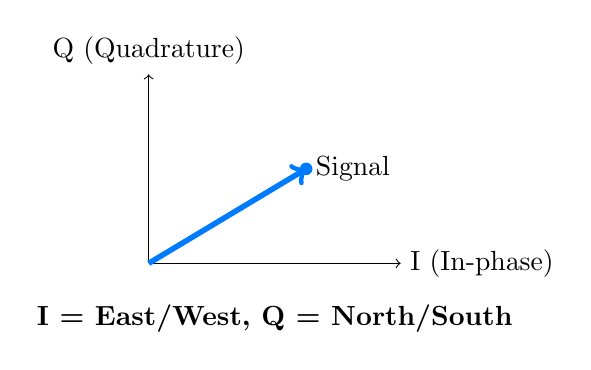
\begin{tikzpicture}[scale=0.8]
    % I and Q representation
    \draw[->] (0,0) -- (4,0) node[right] {I (In-phase)};
    \draw[->] (0,0) -- (0,3) node[above] {Q (Quadrature)};
    \draw[->, radioblue, line width=2pt] (0,0) -- (2.5,1.5);
    \fill[radioblue] (2.5,1.5) circle (0.1);
    \node[right] at (2.5,1.5) {Signal};
    \node[below] at (2,-0.5) {\textbf{I = East/West, Q = North/South}};
\end{tikzpicture}
\end{frame}

\begin{frame}{Sampling: Capturing Radio Waves}
\begin{center}
\Large\textbf{Like Taking Photos of a Moving Object}
\end{center}
\vspace{1em}
\begin{columns}
\column{0.5\textwidth}
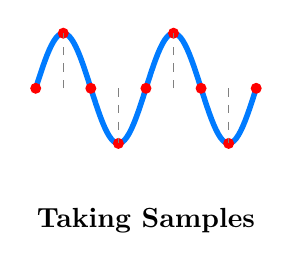
\begin{tikzpicture}[scale=0.7]
    % Original wave
    \draw[radioblue, line width=2pt] plot[domain=0:4, samples=100] (\x, {sin(\x*180)});
    % Sample points
    \foreach \x in {0,0.5,1,1.5,2,2.5,3,3.5,4} {
        \fill[red] (\x,{sin(\x*180)}) circle (0.1);
        \draw[dashed, gray] (\x,0) -- (\x,{sin(\x*180)});
    }
    \node[below] at (2,-2) {\textbf{Taking Samples}};
\end{tikzpicture}

\column{0.5\textwidth}
\textbf{Sampling Rate:}
\begin{itemize}
    \item How often we "photograph"
    \item More samples = Better quality
    \item Like video frame rate
    \item Typical: 2.4 million/second!
\end{itemize}
\end{columns}
\vspace{1em}
\begin{center}\colorbox{yellow!20}{\parbox{0.9\textwidth}{
\textbf{Rule of Thumb:} Sample at least 2x faster than highest frequency\\
(Like needing 60 fps to capture 30 Hz motion smoothly)
}}\end{center}
\end{frame}

\begin{frame}{From Air to Computer - The Journey}
\begin{center}
\Large\textbf{How Radio Waves Become Computer Data}
\end{center}
\vspace{1em}
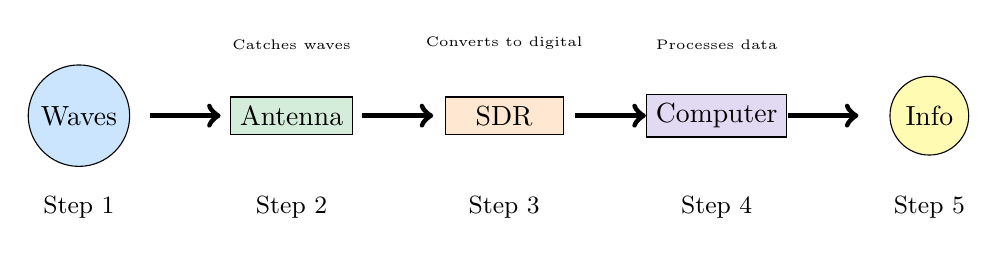
\begin{tikzpicture}[scale=0.9]
    % Step 1: Radio waves
    \node[draw, circle, minimum size=1cm, fill=radioblue!20] (waves) at (0,0) {Waves};
    \node[below] at (0,-1) {\small Step 1};
    
    % Arrow
    \draw[->, line width=2pt] (1,0) -- (2,0);
    
    % Step 2: Antenna
    \node[draw, rectangle, minimum width=1.5cm, fill=radiogreen!20] (antenna) at (3,0) {Antenna};
    \node[below] at (3,-1) {\small Step 2};
    \node[above] at (3,0.8) {\tiny Catches waves};
    
    % Arrow
    \draw[->, line width=2pt] (4,0) -- (5,0);
    
    % Step 3: SDR Hardware
    \node[draw, rectangle, minimum width=1.5cm, fill=radioorange!20] (sdr) at (6,0) {SDR};
    \node[below] at (6,-1) {\small Step 3};
    \node[above] at (6,0.8) {\tiny Converts to digital};
    
    % Arrow
    \draw[->, line width=2pt] (7,0) -- (8,0);
    
    % Step 4: Computer
    \node[draw, rectangle, minimum width=1.5cm, fill=radiopurple!20] (computer) at (9,0) {Computer};
    \node[below] at (9,-1) {\small Step 4};
    \node[above] at (9,0.8) {\tiny Processes data};
    
    % Arrow
    \draw[->, line width=2pt] (10,0) -- (11,0);
    
    % Step 5: Output
    \node[draw, circle, minimum size=1cm, fill=yellow!30] (output) at (12,0) {Info};
    \node[below] at (12,-1) {\small Step 5};
\end{tikzpicture}
\vspace{1em}
\begin{center}
\highlight{Each step is reversible - we can also transmit!}
\end{center}
\end{frame}

\begin{frame}{Why GNU Radio? - Your Swiss Army Knife}
\begin{columns}
\column{0.5\textwidth}
\textbf{\Large GNU Radio Gives You:}
\begin{itemize}
    \item \textcolor{radioblue}{Free and Open Source}
    \item \textcolor{radiogreen}{Visual Programming}
    \item \textcolor{radioorange}{Huge Block Library}
    \item \textcolor{radiopurple}{Active Community}
    \item \textcolor{radiogray}{Works with Any SDR}
    \item \textcolor{radioblue}{Python Integration}
\end{itemize}

\column{0.5\textwidth}
\begin{center}
\textbf{\Large Like Having:}
\end{center}
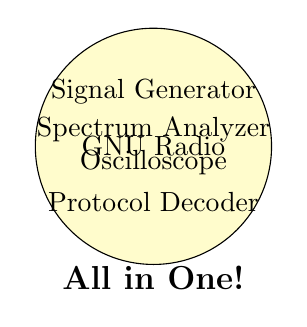
\begin{tikzpicture}[scale=0.7]
    \node[draw, circle, minimum size=3cm, fill=yellow!20] at (0,0) {GNU Radio};
    \node at (0,1) {Signal Generator};
    \node at (0,0.3) {Spectrum Analyzer};
    \node at (0,-0.3) {Oscilloscope};
    \node at (0,-1) {Protocol Decoder};
    \node[below] at (0,-2) {\large\textbf{All in One!}};
\end{tikzpicture}
\end{columns}
\vspace{0.5em}
\begin{center}\colorbox{yellow!20}{\parbox{0.9\textwidth}{
\centering
\large\textbf{Professional tools used by NASA, SpaceX, and researchers worldwide!}
}}\end{center}
\end{frame}

% ============================================
% SECTION 4: VISUAL INTRODUCTION TO GRC
% ============================================

\section{Meet GNU Radio Companion}

\begin{frame}{GRC: Your Radio LEGO Set}
\begin{center}
\Large\textbf{GNU Radio Companion - Where Magic Happens!}
\end{center}
\vspace{1em}
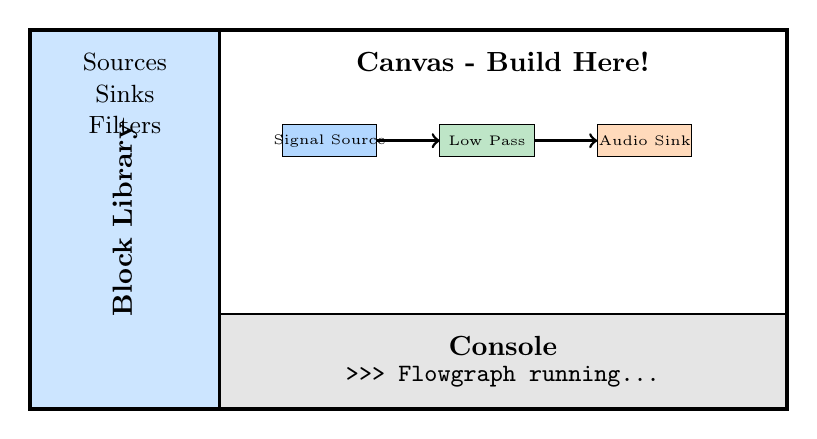
\begin{tikzpicture}[scale=0.8]
    % Main window outline
    \draw[line width=2pt] (0,0) rectangle (12,6);
    
    % Block library
    \draw[line width=1pt, fill=radioblue!20] (0,0) rectangle (3,6);
    \node[rotate=90] at (1.5,3) {\textbf{Block Library}};
    \node at (1.5,5.5) {\small Sources};
    \node at (1.5,5) {\small Sinks};
    \node at (1.5,4.5) {\small Filters};
    
    % Canvas
    \draw[line width=1pt, fill=white] (3,1.5) rectangle (12,6);
    \node at (7.5,5.5) {\textbf{Canvas - Build Here!}};
    % Sample blocks
    \draw[fill=radioblue!30] (4,4) rectangle (5.5,4.5);
    \node at (4.75,4.25) {\tiny Signal Source};
    \draw[fill=radiogreen!30] (6.5,4) rectangle (8,4.5);
    \node at (7.25,4.25) {\tiny Low Pass};
    \draw[fill=radioorange!30] (9,4) rectangle (10.5,4.5);
    \node at (9.75,4.25) {\tiny Audio Sink};
    % Connections
    \draw[->, line width=1pt] (5.5,4.25) -- (6.5,4.25);
    \draw[->, line width=1pt] (8,4.25) -- (9,4.25);
    
    % Console
    \draw[line width=1pt, fill=gray!20] (3,0) rectangle (12,1.5);
    \node at (7.5,1) {\textbf{Console}};
    \node at (7.5,0.5) {\small\texttt{>>> Flowgraph running...}};
\end{tikzpicture}
\vspace{0.5em}
\begin{center}
\highlight{Drag, Drop, Connect - No coding required to start!}
\end{center}
\end{frame}

\begin{frame}{Reading a Flowgraph - Follow the Arrow!}
\begin{center}
\Large\textbf{Flowgraphs Show Signal Path}
\end{center}
\vspace{1em}
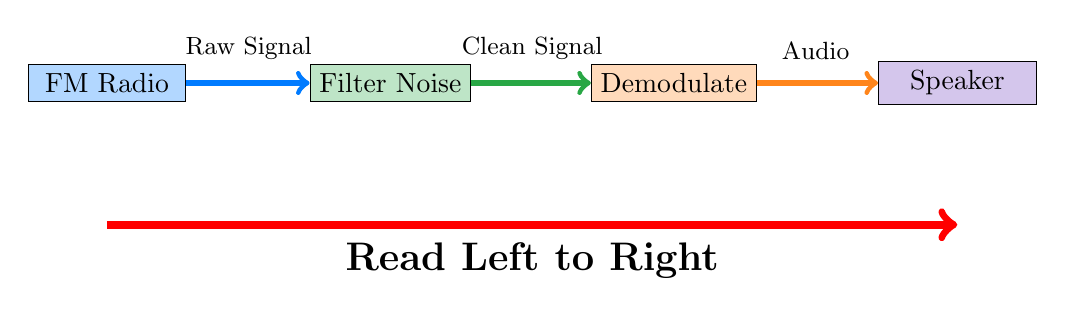
\begin{tikzpicture}[scale=0.9]
    % Example flowgraph
    \node[draw, rectangle, fill=radioblue!30, minimum width=2cm] (source) at (0,0) {FM Radio};
    \node[draw, rectangle, fill=radiogreen!30, minimum width=2cm] (filter) at (4,0) {Filter Noise};
    \node[draw, rectangle, fill=radioorange!30, minimum width=2cm] (demod) at (8,0) {Demodulate};
    \node[draw, rectangle, fill=radiopurple!30, minimum width=2cm] (sink) at (12,0) {Speaker};
    
    \draw[->, line width=2pt, radioblue] (source) -- (filter);
    \node[above] at (2,0.2) {\small Raw Signal};
    
    \draw[->, line width=2pt, radiogreen] (filter) -- (demod);
    \node[above] at (6,0.2) {\small Clean Signal};
    
    \draw[->, line width=2pt, radioorange] (demod) -- (sink);
    \node[above] at (10,0.2) {\small Audio};
    
    % Reading direction
    \draw[->, line width=3pt, red] (0,-2) -- (12,-2);
    \node at (6,-2.5) {\Large\textbf{Read Left to Right}};
\end{tikzpicture}
\vspace{1em}
\begin{columns}
\column{0.33\textwidth}
\centering
\textcolor{radioblue}{\textbf{Start}}\\
Where signal comes from

\column{0.33\textwidth}
\centering
\textcolor{radiogreen}{\textbf{Middle}}\\
Processing steps

\column{0.33\textwidth}
\centering
\textcolor{radioorange}{\textbf{End}}\\
Where signal goes
\end{columns}
\end{frame}

\begin{frame}{Block Colors Mean Something!}
\begin{center}
\Large\textbf{Colors = Data Types (Like Cable Types)}
\end{center}
\vspace{1em}
\begin{columns}
\column{0.5\textwidth}
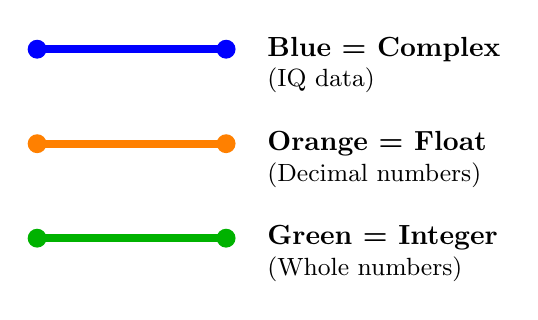
\begin{tikzpicture}[scale=0.8]
    % Blue connection
    \draw[line width=3pt, blue] (0,4) -- (3,4);
    \fill[blue] (0,4) circle (0.15);
    \fill[blue] (3,4) circle (0.15);
    \node[right] at (3.5,4) {\textbf{Blue = Complex}};
    \node[right] at (3.5,3.5) {\small (IQ data)};
    
    % Orange connection
    \draw[line width=3pt, orange] (0,2.5) -- (3,2.5);
    \fill[orange] (0,2.5) circle (0.15);
    \fill[orange] (3,2.5) circle (0.15);
    \node[right] at (3.5,2.5) {\textbf{Orange = Float}};
    \node[right] at (3.5,2) {\small (Decimal numbers)};
    
    % Green connection
    \draw[line width=3pt, green!70!black] (0,1) -- (3,1);
    \fill[green!70!black] (0,1) circle (0.15);
    \fill[green!70!black] (3,1) circle (0.15);
    \node[right] at (3.5,1) {\textbf{Green = Integer}};
    \node[right] at (3.5,0.5) {\small (Whole numbers)};
\end{tikzpicture}

\column{0.5\textwidth}
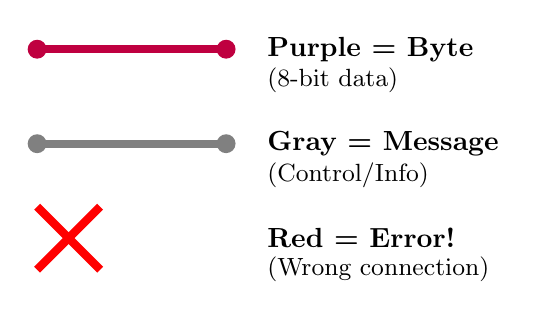
\begin{tikzpicture}[scale=0.8]
    % Purple connection
    \draw[line width=3pt, purple] (0,4) -- (3,4);
    \fill[purple] (0,4) circle (0.15);
    \fill[purple] (3,4) circle (0.15);
    \node[right] at (3.5,4) {\textbf{Purple = Byte}};
    \node[right] at (3.5,3.5) {\small (8-bit data)};
    
    % Gray connection
    \draw[line width=3pt, gray] (0,2.5) -- (3,2.5);
    \fill[gray] (0,2.5) circle (0.15);
    \fill[gray] (3,2.5) circle (0.15);
    \node[right] at (3.5,2.5) {\textbf{Gray = Message}};
    \node[right] at (3.5,2) {\small (Control/Info)};
    
    % Red X
    \draw[line width=3pt, red] (0,0.5) -- (1,1.5);
    \draw[line width=3pt, red] (0,1.5) -- (1,0.5);
    \node[right] at (3.5,1) {\textbf{Red = Error!}};
    \node[right] at (3.5,0.5) {\small (Wrong connection)};
\end{tikzpicture}
\end{columns}
\vspace{1em}
\begin{center}\colorbox{yellow!20}{\parbox{0.9\textwidth}{
\textbf{Golden Rule:} Same colors connect! Different colors = ERROR!
}}\end{center}
\end{frame}

\begin{frame}{Your First 5 Essential Blocks}
\begin{center}
\Large\textbf{Master These First!}
\end{center}
\vspace{0.5em}
\begin{columns}
\column{0.5\textwidth}
\textbf{1. Signal Source}
\begin{itemize}
    \item Creates test signals
    \item Sine, Square, Sawtooth
    \item Set frequency \& amplitude
\end{itemize}
\vspace{0.5em}
\textbf{2. Audio Source/Sink}
\begin{itemize}
    \item Microphone input
    \item Speaker output
    \item Real-world connection
\end{itemize}

\column{0.5\textwidth}
\textbf{3. QT GUI Time Sink}
\begin{itemize}
    \item See signal over time
    \item Like oscilloscope
    \item Visual feedback
\end{itemize}
\vspace{0.5em}
\textbf{4. Throttle}
\begin{itemize}
    \item Controls data rate
    \item Prevents CPU overload
    \item \textcolor{red}{Always use in simulation!}
\end{itemize}
\end{columns}
\vspace{0.5em}
\begin{center}
\textbf{5. File Source/Sink}
\begin{itemize}
    \item Save/load signals
    \item Record for later
    \item Share with others
\end{itemize}
\end{center}
\end{frame}

\begin{frame}{Common Patterns - Copy These!}
\begin{center}
\Large\textbf{Starter Templates}
\end{center}
\vspace{0.5em}

\textbf{Pattern 1: Signal Generator}
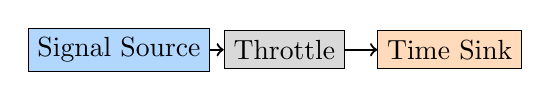
\begin{tikzpicture}[scale=0.7]
    \node[draw, fill=radioblue!30] (src) at (0,0) {Signal Source};
    \node[draw, fill=gray!30] (thr) at (3,0) {Throttle};
    \node[draw, fill=radioorange!30] (sink) at (6,0) {Time Sink};
    \draw[->, thick] (src) -- (thr);
    \draw[->, thick] (thr) -- (sink);
\end{tikzpicture}

\vspace{0.5em}
\textbf{Pattern 2: Audio Processor}
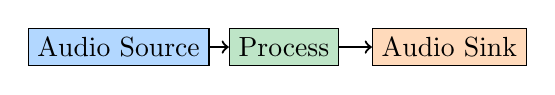
\begin{tikzpicture}[scale=0.7]
    \node[draw, fill=radioblue!30] (src) at (0,0) {Audio Source};
    \node[draw, fill=radiogreen!30] (proc) at (3,0) {Process};
    \node[draw, fill=radioorange!30] (sink) at (6,0) {Audio Sink};
    \draw[->, thick] (src) -- (proc);
    \draw[->, thick] (proc) -- (sink);
\end{tikzpicture}

\vspace{0.5em}
\textbf{Pattern 3: File Playback}
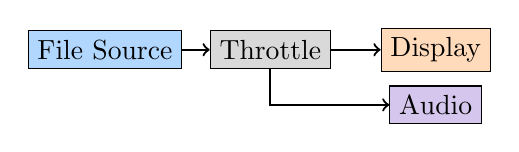
\begin{tikzpicture}[scale=0.7]
    \node[draw, fill=radioblue!30] (src) at (0,0) {File Source};
    \node[draw, fill=gray!30] (thr) at (3,0) {Throttle};
    \node[draw, fill=radioorange!30] (sink1) at (6,0) {Display};
    \node[draw, fill=radiopurple!30] (sink2) at (6,-1) {Audio};
    \draw[->, thick] (src) -- (thr);
    \draw[->, thick] (thr) -- (sink1);
    \draw[->, thick] (thr) |- (sink2);
\end{tikzpicture}

\begin{center}
\highlight{Start with these patterns and modify!}
\end{center}
\end{frame}

\begin{frame}{Making Connections - The Rules}
\begin{center}
\Large\textbf{Connection Rules - Simple!}
\end{center}
\vspace{1em}
\begin{columns}
\column{0.5\textwidth}
\textcolor{green}{\Large\textbf{$\checkmark$ DO This:}}
\begin{itemize}
    \item Match colors
    \item One output to many inputs
    \item Use Throttle in simulations
    \item Connect all outputs
\end{itemize}
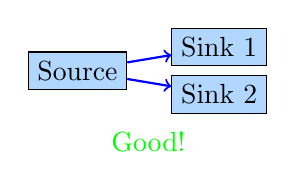
\begin{tikzpicture}[scale=0.6]
    \node[draw, fill=radioblue!30] (src) at (0,0) {Source};
    \node[draw, fill=radioblue!30] (sink1) at (3,0.5) {Sink 1};
    \node[draw, fill=radioblue!30] (sink2) at (3,-0.5) {Sink 2};
    \draw[->, thick, blue] (src) -- (sink1);
    \draw[->, thick, blue] (src) -- (sink2);
    \node at (1.5,-1.5) {\textcolor{green}{Good!}};
\end{tikzpicture}

\column{0.5\textwidth}
\textcolor{red}{\Large\textbf{$\times$ DON'T Do This:}}
\begin{itemize}
    \item Mix colors
    \item Many outputs to one input
    \item Forget Throttle
    \item Leave blocks unconnected
\end{itemize}
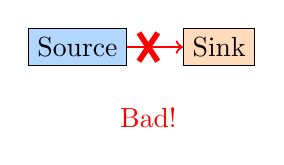
\begin{tikzpicture}[scale=0.6]
    \node[draw, fill=radioblue!30] (src) at (0,0) {Source};
    \node[draw, fill=radioorange!30] (sink) at (3,0) {Sink};
    \draw[->, thick, red] (src) -- (sink);
    \draw[red, line width=2pt] (1.3,-0.3) -- (1.7,0.3);
    \draw[red, line width=2pt] (1.3,0.3) -- (1.7,-0.3);
    \node at (1.5,-1.5) {\textcolor{red}{Bad!}};
\end{tikzpicture}
\end{columns}
\vspace{1em}
\tryitnow{
Draw a simple flowgraph on paper: Signal Source → Throttle → Display
}
\end{frame}

\begin{frame}{Avoiding Common Beginner Mistakes}
\begin{center}
\Large\textbf{Top 5 Mistakes and How to Fix Them}
\end{center}
\vspace{0.5em}
\begin{enumerate}
    \item \textbf{\textcolor{red}{Forgetting Throttle Block}}\\
    \textcolor{green}{Fix:} Always add Throttle when not using hardware\\[0.5em]
    
    \item \textbf{\textcolor{red}{Wrong Sample Rates}}\\
    \textcolor{green}{Fix:} Keep sample rates consistent (use variables!)\\[0.5em]
    
    \item \textbf{\textcolor{red}{Type Mismatch (Red Errors)}}\\
    \textcolor{green}{Fix:} Check port colors match exactly\\[0.5em]
    
    \item \textbf{\textcolor{red}{No Output/Display}}\\
    \textcolor{green}{Fix:} Check connections and GUI hints\\[0.5em]
    
    \item \textbf{\textcolor{red}{CPU at 100\%}}\\
    \textcolor{green}{Fix:} Add Throttle, reduce sample rate
\end{enumerate}
\vspace{0.5em}
\begin{center}\colorbox{yellow!20}{\parbox{0.9\textwidth}{
\textbf{Pro Tip:} Check the console for error messages - they're helpful!
}}\end{center}
\end{frame}

% ============================================
% SECTION 5: HANDS-ON PREPARATION
% ============================================

\section{Let's Build Something!}

\begin{frame}{What You'll Build Today}
\begin{center}
\Large\textbf{Your Workshop Projects}
\end{center}
\vspace{1em}
\begin{columns}
\column{0.25\textwidth}
\begin{center}
\includegraphics[width=\textwidth]{images/project1.png}
\textbf{Project 1}\\
\textcolor{radioblue}{Dial Tone}\\
\small 15 minutes
\end{center}

\column{0.25\textwidth}
\begin{center}
\includegraphics[width=\textwidth]{images/project2.png}
\textbf{Project 2}\\
\textcolor{radiogreen}{FM Receiver}\\
\small 30 minutes
\end{center}

\column{0.25\textwidth}
\begin{center}
\includegraphics[width=\textwidth]{images/project3.png}
\textbf{Project 3}\\
\textcolor{radioorange}{Spectrum Analyzer}\\
\small 30 minutes
\end{center}

\column{0.25\textwidth}
\begin{center}
\includegraphics[width=\textwidth]{images/project4.png}
\textbf{Project 4}\\
\textcolor{radiopurple}{Digital Decoder}\\
\small 45 minutes
\end{center}
\end{columns}
\vspace{1em}
\begin{center}
\Large\highlight{Each builds on the previous - you'll be an expert by day's end!}
\end{center}
\end{frame}

\begin{frame}{Tools We'll Use}
\begin{columns}
\column{0.5\textwidth}
\textbf{\Large Software:}
\begin{itemize}
    \item GNU Radio Companion (GRC)
    \item Python (optional)
    \item Text Editor
    \item Terminal/Command Line
\end{itemize}
\vspace{1em}
\textbf{\Large Files Provided:}
\begin{itemize}
    \item Example flowgraphs
    \item Sample recordings
    \item Python templates
    \item Quick reference guide
\end{itemize}

\column{0.5\textwidth}
\textbf{\Large Hardware (Optional):}
\begin{itemize}
    \item RTL-SDR (\$30)
    \item Antenna
    \item USB cable
    \item Computer with USB port
\end{itemize}
\vspace{1em}
\textbf{\Large No Hardware? No Problem!}
\begin{itemize}
    \item Use provided recordings
    \item Simulate everything
    \item Borrow from neighbor
    \item Watch demos
\end{itemize}
\end{columns}
\end{frame}

\begin{frame}{Getting Help During Workshop}
\begin{center}
\Large\textbf{We're Here to Help!}
\end{center}
\vspace{1em}
\begin{columns}
\column{0.5\textwidth}
\textbf{When Stuck:}
\begin{enumerate}
    \item Raise your hand
    \item Check console messages
    \item Ask your neighbor
    \item Reference the guide
    \item Don't worry - it's normal!
\end{enumerate}

\column{0.5\textwidth}
\textbf{Help Signals:}
\begin{itemize}
    \item \textcolor{red}{Red Card:} I'm stuck
    \item \textcolor{yellow}{Yellow Card:} Question
    \item \textcolor{green}{Green Card:} I'm good
\end{itemize}
\vspace{1em}
\textbf{Online Help:}
\begin{itemize}
    \item Workshop chat channel
    \item Quick reference PDF
    \item Example solutions
\end{itemize}
\end{columns}
\vspace{1em}
\begin{center}\colorbox{yellow!20}{\parbox{0.9\textwidth}{
\centering
\large\textbf{No question is too simple - we all started here!}
}}\end{center}
\end{frame}

\begin{frame}{Let's Test Your Setup!}
\begin{center}
\Large\textbf{Quick Setup Check}
\end{center}
\vspace{1em}
\tryitnow{
Follow along - we'll do this together!
}
\vspace{1em}
\begin{enumerate}
    \item \textbf{Open Terminal/Command Prompt}
    \begin{itemize}
        \item Type: \texttt{gnuradio-companion}
        \item Press Enter
    \end{itemize}
    
    \item \textbf{GRC Should Open}
    \begin{itemize}
        \item See the interface?
        \item If not, raise red card!
    \end{itemize}
    
    \item \textbf{Create Test Flowgraph}
    \begin{itemize}
        \item Add: Signal Source
        \item Add: Throttle
        \item Add: QT GUI Time Sink
        \item Connect them
    \end{itemize}
    
    \item \textbf{Run It!}
    \begin{itemize}
        \item Press F6 or click Run
        \item See a sine wave?
        \item Success! Green card up!
    \end{itemize}
\end{enumerate}
\end{frame}

% ============================================
% SECTION 6: INTERACTIVE DEMOS
% ============================================

\section{Live Demonstrations}

% Temporarily commenting out problematic frame
\iffalse
\begin{frame}{Demo 1: Your First Signal}
\begin{center}
\Large\textbf{Let's Make a Beep!}
\end{center}
\vspace{1em}
\begin{columns}
\column{0.5\textwidth}
\textbf{Steps:}
\begin{enumerate}
    \item Open GRC
    \item Add Signal Source
    \item Set to 440 Hz (A note)
    \item Add Audio Sink
    \item Connect them
    \item Run!
\end{enumerate}

\column{0.5\textwidth}
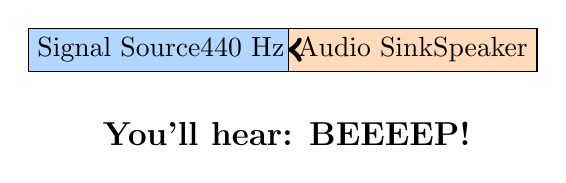
\begin{tikzpicture}[scale=0.8]
    \node[draw, rectangle, fill=radioblue!30, minimum width=2cm] (source) at (0,0) {Signal Source\\440 Hz};
    \node[draw, rectangle, fill=radioorange!30, minimum width=2cm] (sink) at (4,0) {Audio Sink\\Speaker};
    \draw[->, line width=2pt] (source) -- (sink);
    
    \node[below] at (2,-1) {\large\textbf{You'll hear: BEEEEP!}};
\end{tikzpicture}
\end{columns}

\vspace{1em}
\begin{center}
\colorbox{yellow!20}{\parbox{0.9\textwidth}{\centering
\textbf{Experiment:} Change frequency to 880 Hz - what happens to the pitch?}}
\end{center}
\end{frame}
\fi

\begin{frame}{Demo 2: FM Radio Receiver}
\begin{center}
\Large\textbf{Listen to Real Radio!}
\end{center}
\vspace{0.5em}
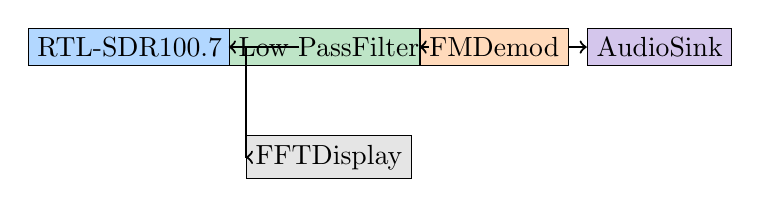
\begin{tikzpicture}[scale=0.7]
    \node[draw, fill=radioblue!30, minimum width=1.5cm] (rtl) at (0,0) {RTL-SDR\\100.7 MHz};
    \node[draw, fill=radiogreen!30, minimum width=1.5cm] (lpf) at (3,0) {Low Pass\\Filter};
    \node[draw, fill=radioorange!30, minimum width=1.5cm] (fm) at (6,0) {FM\\Demod};
    \node[draw, fill=radiopurple!30, minimum width=1.5cm] (audio) at (9,0) {Audio\\Sink};
    
    \draw[->, thick] (rtl) -- (lpf);
    \draw[->, thick] (lpf) -- (fm);
    \draw[->, thick] (fm) -- (audio);
    
    % Spectrum display
    \node[draw, fill=gray!20, minimum width=1.5cm] (fft) at (3,-2) {FFT\\Display};
    \draw[->, thick] (1.5,0) |- (fft);
\end{tikzpicture}

\vspace{0.5em}
\begin{minipage}{\textwidth}
\textbf{What You'll See/Hear:}
\begin{itemize}
    \item Spectrum display shows radio stations
    \item Audio plays through speakers
    \item Can tune to different stations
    \item See signal strength change
\end{itemize}
\end{minipage}
\vspace{0.5em}
\begin{center}
\highlight{No hardware? Use provided FM recording file!}
\end{center}
\end{frame}

\begin{frame}{Demo 3: See Your Voice}
\begin{center}
\Large\textbf{Visualize Your Voice in Real-Time!}
\end{center}
\vspace{1em}
\begin{columns}
\column{0.5\textwidth}
\begin{minipage}{\textwidth}
\textbf{Build This:}
\begin{enumerate}
    \item Audio Source (Mic)
    \item QT GUI Time Sink
    \item QT GUI Frequency Sink
    \item Connect both displays
\end{enumerate}
\end{minipage}
\vspace{0.5em}
\begin{minipage}{\textwidth}
\textbf{Try Speaking:}
\begin{itemize}
    \item "Ahhhhh" - steady tone
    \item "Sssss" - high frequency
    \item Whistle - pure tone
    \item Clap - impulse
\end{itemize}
\end{minipage}

\column{0.5\textwidth}
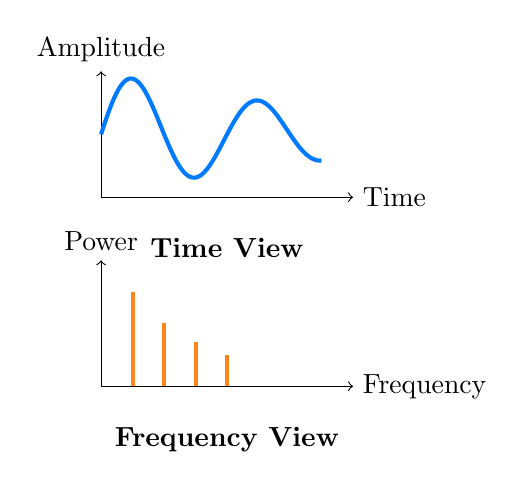
\begin{tikzpicture}[scale=0.8]
    % Time domain
    \draw[->] (0,0) -- (4,0) node[right] {Time};
    \draw[->] (0,0) -- (0,2) node[above] {Amplitude};
    \draw[radioblue, line width=1.5pt] plot[domain=0:3.5, samples=100] (\x, {sin(\x*180)*exp(-\x/4) + 1});
    \node[below] at (2,-0.5) {\textbf{Time View}};
    
    % Frequency domain
    \draw[->] (0,-3) -- (4,-3) node[right] {Frequency};
    \draw[->] (0,-3) -- (0,-1) node[above] {Power};
    \draw[radioorange, line width=1.5pt] (0.5,-3) -- (0.5,-1.5);
    \draw[radioorange, line width=1.5pt] (1,-3) -- (1,-2);
    \draw[radioorange, line width=1.5pt] (1.5,-3) -- (1.5,-2.3);
    \draw[radioorange, line width=1.5pt] (2,-3) -- (2,-2.5);
    \node[below] at (2,-3.5) {\textbf{Frequency View}};
\end{tikzpicture}
\end{columns}
\end{frame}

\begin{frame}{Demo 4: Decode a Digital Message}
\begin{center}
\Large\textbf{From Beeps to Text!}
\end{center}
\vspace{1em}
\begin{columns}
\column{0.6\textwidth}
\textbf{Digital Communication Chain:}
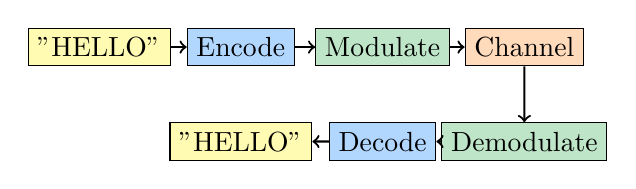
\begin{tikzpicture}[scale=0.6]
    \node[draw, fill=yellow!30] (text) at (0,0) {"HELLO"};
    \node[draw, fill=radioblue!30] (enc) at (3,0) {Encode};
    \node[draw, fill=radiogreen!30] (mod) at (6,0) {Modulate};
    \node[draw, fill=radioorange!30] (chan) at (9,0) {Channel};
    \node[draw, fill=radiogreen!30] (demod) at (9,-2) {Demodulate};
    \node[draw, fill=radioblue!30] (dec) at (6,-2) {Decode};
    \node[draw, fill=yellow!30] (out) at (3,-2) {"HELLO"};
    
    \draw[->, thick] (text) -- (enc);
    \draw[->, thick] (enc) -- (mod);
    \draw[->, thick] (mod) -- (chan);
    \draw[->, thick] (chan) -- (demod);
    \draw[->, thick] (demod) -- (dec);
    \draw[->, thick] (dec) -- (out);
\end{tikzpicture}

\column{0.4\textwidth}
\textbf{You'll Learn:}
\begin{itemize}
    \item Binary = 0s and 1s
    \item Modulation = Pattern
    \item Demodulation = Decode
    \item Error correction
\end{itemize}
\end{columns}
\vspace{1em}
\begin{center}
\highlight{We'll send "HELLO WORLD" through the air (or simulation)!}
\end{center}
\end{frame}

\begin{frame}{Challenge Preview}
\begin{center}
\Large\textbf{By End of Day, You'll Complete These Challenges!}
\end{center}
\vspace{1em}
\begin{columns}
\column{0.5\textwidth}
\textbf{Morning Challenges:}
\begin{itemize}
    \item Build an FM radio
    \item Create audio effects
    \item Design filters
    \item Analyze spectrum
\end{itemize}

\column{0.5\textwidth}
\textbf{Afternoon Challenges:}
\begin{itemize}
    \item Decode aircraft data
    \item Build walkie-talkie
    \item Create custom block
    \item Design protocol
\end{itemize}
\end{columns}
\vspace{1em}
\begin{center}\colorbox{yellow!20}{\parbox{0.9\textwidth}{
\centering
\Large\textbf{Grand Challenge: Build Your Own Application!}\\
\normalsize Choose your project and we'll help you build it!
}}\end{center}
\end{frame}

% ============================================
% SECTION 7: CONCEPTUAL BRIDGING
% ============================================

\section{Next Steps}

\begin{frame}{From Blocks to Code}
\begin{center}
\Large\textbf{GRC Creates Python Code for You!}
\end{center}
\vspace{1em}
\begin{columns}
\column{0.5\textwidth}
\textbf{What You See (GRC):}
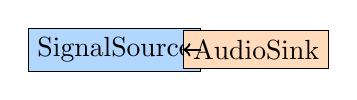
\begin{tikzpicture}[scale=0.6]
    \node[draw, fill=radioblue!30] (src) at (0,0) {Signal\\Source};
    \node[draw, fill=radioorange!30] (sink) at (3,0) {Audio\\Sink};
    \draw[->, thick] (src) -- (sink);
\end{tikzpicture}

\column{0.5\textwidth}
\textbf{What It Becomes (Python):}
\begin{verbatim}
source = analog.sig_source()
sink = audio.sink()
connect(source, sink)
\end{verbatim}
\end{columns}
\vspace{1em}
\begin{center}
\Large\highlight{Visual programming becomes real code automatically!}
\end{center}
\vspace{0.5em}
\begin{itemize}
    \item Press "Generate" button
    \item Creates .py file
    \item Can edit and customize
    \item Add your own features
\end{itemize}
\end{frame}

\begin{frame}{When to Use GRC vs Python}
\begin{center}
\Large\textbf{Choose the Right Tool}
\end{center}
\vspace{1em}
\begin{columns}
\column{0.5\textwidth}
\textbf{Use GRC When:}
\begin{itemize}
    \item \textcolor{radiogreen}{$\checkmark$} Learning/Prototyping
    \item \textcolor{radiogreen}{$\checkmark$} Visual design needed
    \item \textcolor{radiogreen}{$\checkmark$} Quick experiments
    \item \textcolor{radiogreen}{$\checkmark$} Teaching others
    \item \textcolor{radiogreen}{$\checkmark$} Standard blocks work
\end{itemize}

\column{0.5\textwidth}
\textbf{Use Python When:}
\begin{itemize}
    \item \textcolor{radioblue}{$\checkmark$} Custom processing
    \item \textcolor{radioblue}{$\checkmark$} Complex logic
    \item \textcolor{radioblue}{$\checkmark$} Integration needed
    \item \textcolor{radioblue}{$\checkmark$} Automation required
    \item \textcolor{radioblue}{$\checkmark$} Production system
\end{itemize}
\end{columns}
\vspace{1em}
\begin{center}\colorbox{yellow!20}{\parbox{0.9\textwidth}{
\textbf{Best Practice:} Start in GRC, then generate Python and customize!
}}\end{center}
\end{frame}

\begin{frame}{Real-World Applications}
\begin{center}
\Large\textbf{Where SDR is Used Today}
\end{center}
\vspace{0.5em}
\begin{columns}
\column{0.33\textwidth}
\textbf{Communications:}
\begin{itemize}
    \item 5G/6G Networks
    \item Satellite Internet
    \item Emergency Radio
    \item Maritime Systems
\end{itemize}

\column{0.33\textwidth}
\textbf{Science:}
\begin{itemize}
    \item Radio Astronomy
    \item Weather Satellites
    \item Wildlife Tracking
    \item Ocean Monitoring
\end{itemize}

\column{0.33\textwidth}
\textbf{Security:}
\begin{itemize}
    \item Signal Intelligence
    \item Drone Detection
    \item Interference Hunt
    \item Network Security
\end{itemize}
\end{columns}
\vspace{0.5em}
\begin{columns}
\column{0.33\textwidth}
\textbf{Transportation:}
\begin{itemize}
    \item Aircraft Radar
    \item GPS Systems
    \item Train Control
    \item Ship Navigation
\end{itemize}

\column{0.33\textwidth}
\textbf{IoT/Smart:}
\begin{itemize}
    \item Smart Cities
    \item Agriculture
    \item Health Monitors
    \item Home Automation
\end{itemize}

\column{0.33\textwidth}
\textbf{Entertainment:}
\begin{itemize}
    \item Digital TV
    \item Streaming Radio
    \item Gaming Controllers
    \item VR Systems
\end{itemize}
\end{columns}
\end{frame}

\begin{frame}{Your Learning Path}
\begin{center}
\Large\textbf{Your SDR Journey Roadmap}
\end{center}
\vspace{0.5em}
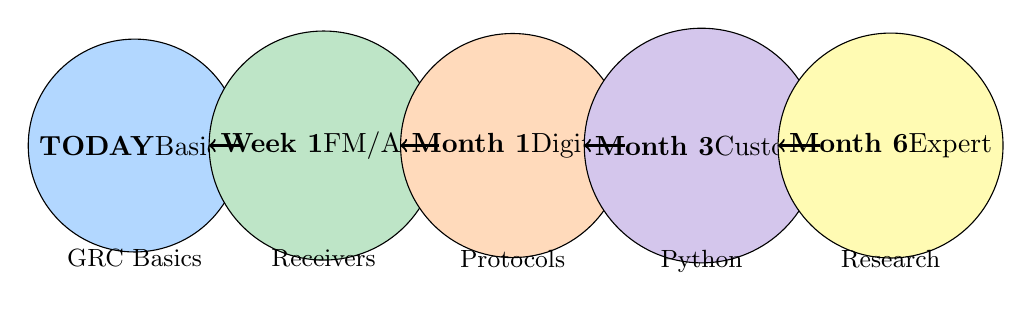
\begin{tikzpicture}[scale=0.8]
    % Today
    \node[draw, circle, fill=radioblue!30, minimum size=1.5cm] (today) at (0,0) {\textbf{TODAY}\\Basics};
    
    % Week 1
    \node[draw, circle, fill=radiogreen!30, minimum size=1.5cm] (week1) at (3,0) {\textbf{Week 1}\\FM/AM};
    \draw[->, thick] (today) -- (week1);
    
    % Month 1
    \node[draw, circle, fill=radioorange!30, minimum size=1.5cm] (month1) at (6,0) {\textbf{Month 1}\\Digital};
    \draw[->, thick] (week1) -- (month1);
    
    % Month 3
    \node[draw, circle, fill=radiopurple!30, minimum size=1.5cm] (month3) at (9,0) {\textbf{Month 3}\\Custom};
    \draw[->, thick] (month1) -- (month3);
    
    % Month 6
    \node[draw, circle, fill=yellow!30, minimum size=1.5cm] (month6) at (12,0) {\textbf{Month 6}\\Expert};
    \draw[->, thick] (month3) -- (month6);
    
    % Skills below
    \node[below] at (0,-1.5) {\small GRC Basics};
    \node[below] at (3,-1.5) {\small Receivers};
    \node[below] at (6,-1.5) {\small Protocols};
    \node[below] at (9,-1.5) {\small Python};
    \node[below] at (12,-1.5) {\small Research};
\end{tikzpicture}
\vspace{1em}
\textbf{Recommended Learning Resources:}
\begin{itemize}
    \item GNU Radio Tutorials (wiki.gnuradio.org)
    \item PySDR Online Book (pysdr.org)
    \item YouTube: GNU Radio channel
    \item Local ham radio clubs
\end{itemize}
\end{frame}

\begin{frame}{Community and Resources}
\begin{center}
\Large\textbf{Join the GNU Radio Family!}
\end{center}
\vspace{1em}
\begin{columns}
\column{0.5\textwidth}
\textbf{Online Communities:}
\begin{itemize}
    \item \textbf{Chat:} chat.gnuradio.org
    \item \textbf{Forum:} discuss.gnuradio.org
    \item \textbf{Reddit:} r/gnuradio
    \item \textbf{Discord:} GNU Radio server
\end{itemize}
\vspace{0.5em}
\textbf{Learning Resources:}
\begin{itemize}
    \item Official tutorials
    \item Video courses
    \item Example flowgraphs
    \item Blog posts
\end{itemize}

\column{0.5\textwidth}
\textbf{Events:}
\begin{itemize}
    \item \textbf{GRCon:} Annual conference
    \item \textbf{Hackathons:} Build together
    \item \textbf{Workshops:} Like this one!
    \item \textbf{Meetups:} Local groups
\end{itemize}
\vspace{0.5em}
\textbf{Contributing:}
\begin{itemize}
    \item Share your projects
    \item Help newcomers
    \item Report bugs
    \item Write tutorials
\end{itemize}
\end{columns}
\vspace{1em}
\begin{center}\colorbox{yellow!20}{\parbox{0.9\textwidth}{
\centering
\large\textbf{Everyone started as a beginner - pay it forward!}
}}\end{center}
\end{frame}

% ============================================
% CLOSING
% ============================================

\begin{frame}{You're Ready!}
\begin{center}
\Huge\textcolor{radioblue}{Let's Start Building!}
\end{center}
\vspace{1em}
\begin{center}
\Large
\textbf{Remember:}
\begin{itemize}
    \item It's okay to make mistakes
    \item Ask questions freely
    \item Help your neighbors
    \item Have fun exploring!
\end{itemize}
\end{center}
\vspace{1em}
\begin{center}
\Large\highlight{Welcome to the world of Software Defined Radio!}
\end{center}
\end{frame}

\begin{frame}{Quick Reference}
\begin{center}
\Large\textbf{Keep This Handy!}
\end{center}
\vspace{0.5em}
\begin{columns}
\column{0.5\textwidth}
\textbf{Keyboard Shortcuts:}
\begin{itemize}
    \item \textbf{F5/F6:} Run flowgraph
    \item \textbf{F7:} Stop flowgraph
    \item \textbf{Ctrl+Z:} Undo
    \item \textbf{Delete:} Remove block
    \item \textbf{R:} Rotate block
\end{itemize}

\column{0.5\textwidth}
\textbf{Common Values:}
\begin{itemize}
    \item Audio rate: 48000
    \item RTL-SDR max: 2.4M
    \item FM bandwidth: 200k
    \item Common gains: 0-50 dB
    \item Throttle: Match sample rate
\end{itemize}
\end{columns}
\vspace{0.5em}
\textbf{Troubleshooting:}
\begin{itemize}
    \item Red error? → Check connections
    \item No output? → Add Throttle
    \item CPU 100\%? → Reduce sample rate
    \item Can't hear? → Check audio device
\end{itemize}
\end{frame}

\end{document}